% Model - med figur
% Algorithm - som figur
% Animationer
% Demo af sumo

\section{Solution}
\begin{frame}{Model}
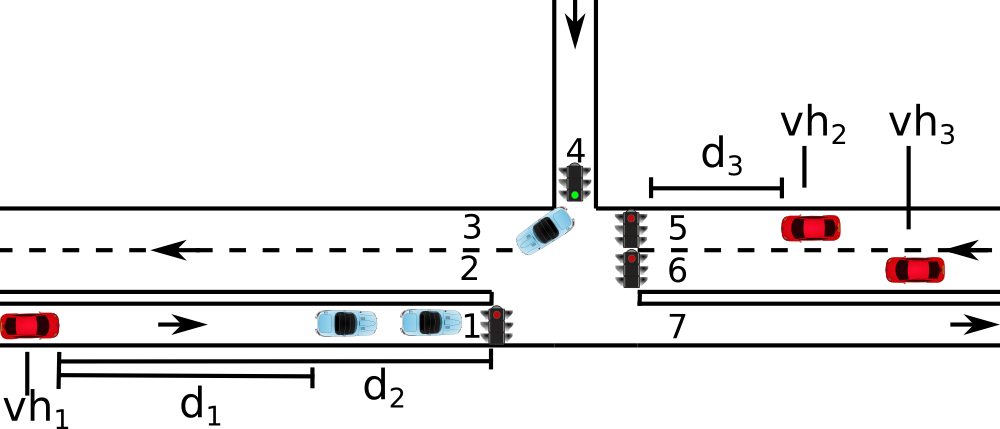
\includegraphics[width=1\textwidth]{images/introNetwork.png}
\end{frame}

\begin{frame}{Space Model}
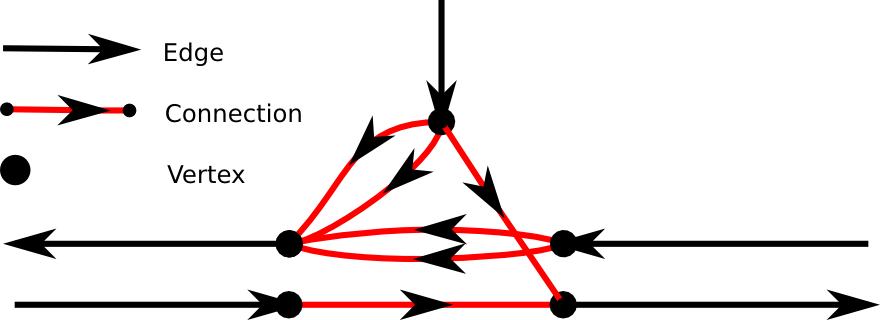
\includegraphics[width=1\textwidth]{images/ConnectionNetwork.png}
\end{frame}

\begin{frame}{Algorithm}
\begin{center}
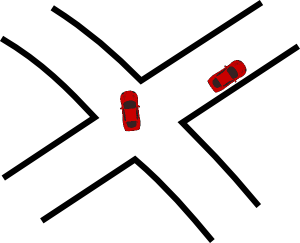
\includegraphics[width=0.8\textwidth]{images/algjuction.png}
\end{center}
\end{frame}

\begin{frame}{Algorithm}
\begin{center}
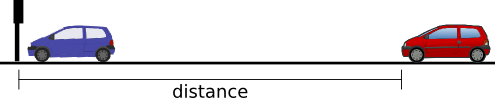
\includegraphics[width=1\textwidth]{images/algdistance.png}
\end{center}
\end{frame}

\begin{frame}{Algorithm}
\begin{columns}
\begin{column}{0.5\textwidth}
\begin{center}
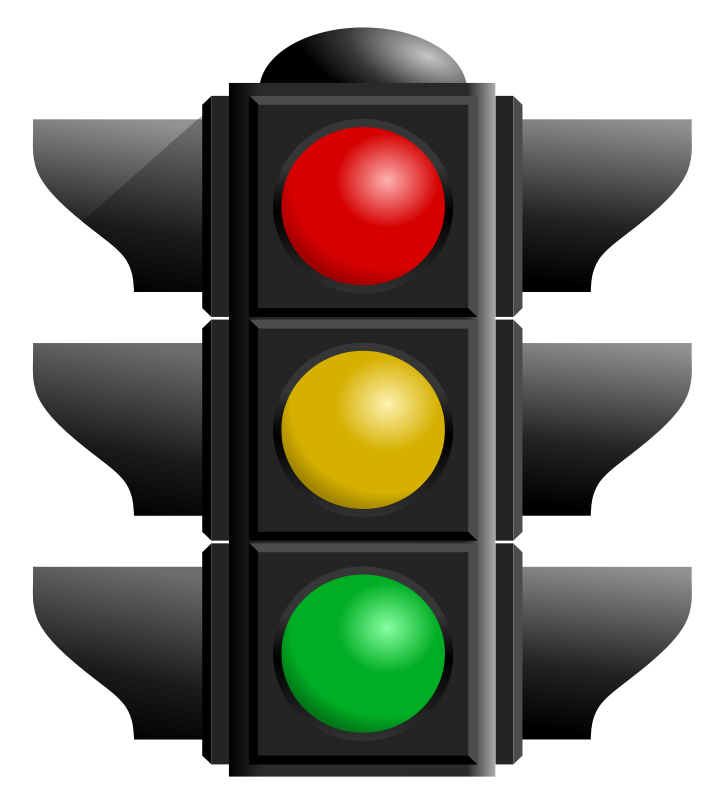
\includegraphics[width=0.7\textwidth]{images/traffic_light.png}
\end{center}
\end{column}
\begin{column}{0.5\textwidth}
\begin{center}
\begin{tabular}{lll}
\textbf{Phase:}&&\\
green & : & 30 s \\
yellow & : &  4 s \\
red & : & 15 s \\
yellow & : & 2 s \\
green & : & 30 s\\
\ \ \ \vdots&&\\
\end{tabular}
\end{center}
\end{column}
\end{columns}
\end{frame}

\begin{frame}{Algorithm}
\[velocity = \frac{distance}{time}\]
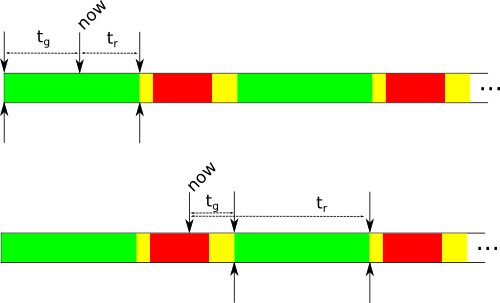
\includegraphics[width=1\textwidth]{images/algphases.png}
\end{frame}







